\subsection{Versuchsaufbau}
\label{sec:Versuchsaufbau}
%\begin{figure}
%	\centering
%	\caption{Schematische Darstellung des Versuchsaufbaus \cite{anleitung}.}
%	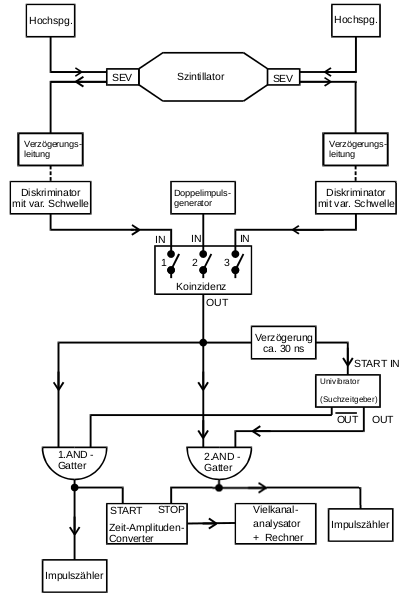
\includegraphics{Bilder/aufbau.png}
%	\label{fig:aufbau}
%\end{figure}
%
%\begin{figure}
%	\centering
%	\caption{Schematische Darstellung der Quelle zur Erzeugung radioaktiven Isotopen \cite{anleitung}.}
%	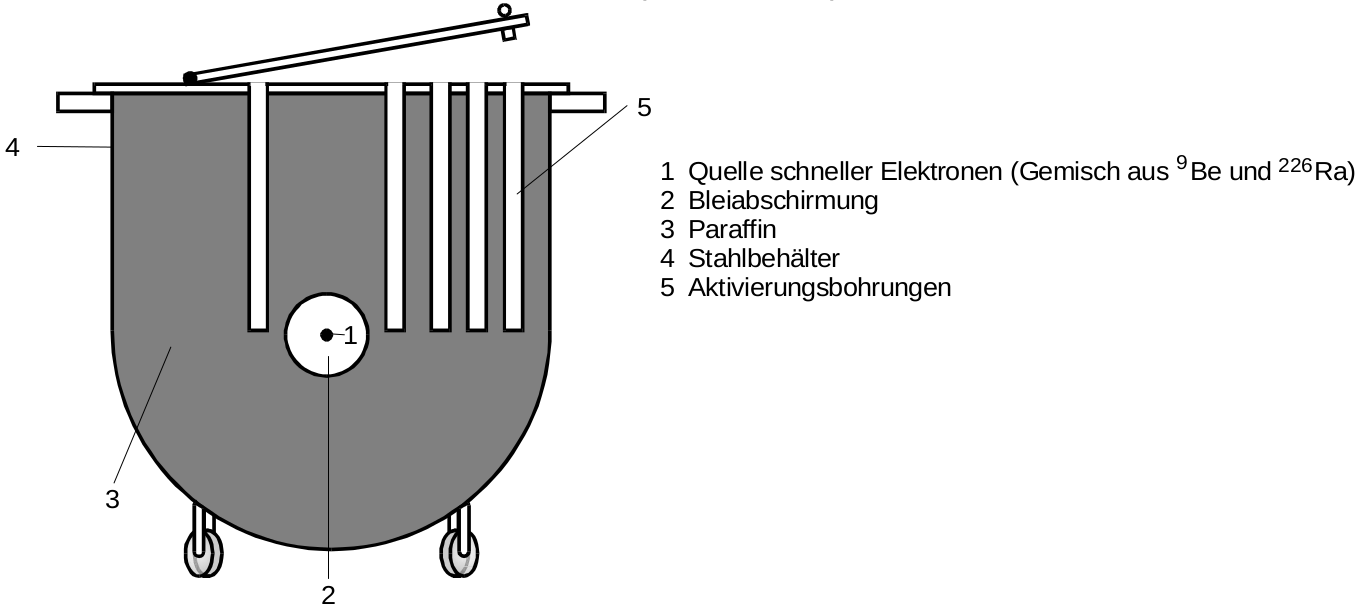
\includegraphics{content/toepfchen.png}
%	\label{fig:kochen}
%\end{figure}
%
Der Versuchsaufbau -- wie in Abbildung \ref{fig:aufbau} dargestellt -- besteht im Wesentlichen 
aus einem zerfallenden radioaktiven Isotop und einem Geiger-Müller-Zählrohr, welches die 
zerfallenden Kerne misst.
Das Geiger-Müller-Zählrohr ist entspricht einer mit Gas gefüllten Röhre. Trifft ein $\beta$-
oder $\gamma$- Teilchen auf ein Gasteilchen wird dieses ionisiert und kann aufgrund einer
anliegenden Spannung an der Röhre gemessen werden.
Dabei werden die gemessenen Zerfälle pro Messzeitintervall, welches am Zeitgeber einstellbar 
ist, an den Zählern 1 und 2 angezeigt. Nach jedem Messvorgang wird der Zähler umgeschaltet und 
der vorherige Wert auf dem aktuellen Zähler wird überschrieben. Der Versuchsaufbau ist mit
einer Blei-Abschirmung ausgestattet um die radioaktive Strahlung abzuschirmen.

Zur Erzeugung der radioaktiven Isotope wird das Objekt in Abbildung \ref{fig:kochen} verwendet.
Hierbei werden stabile Kerne mit niederenergetischen Neutronen beschossen. 
Da die Neutronen ihre Energie durch elastische Stöße an die Kerne übergeben und die maximale
Energie bei gleichen Massen der Stoßpartner erreicht wird, werden die Neutronen in einem 
Paraffinmantel gebremst, bis sie die optimale Energie besitzen.

\section{Durchführung}
\label{sec:Durchführung}
\subsection{Bestimmung der Periodendauer zur Berechnung der elastischen Konstanten}
Zur Messung der Periodendauer zur Berechnung des Schubmoduls $G$ wird der Magnet in der Kugelmasse vertikal ausgerichtet. Dadurch steht der Magnet senkrecht auf der horizontalen Komponente des Erdmagnetfelds und wird durch diese somit nicht beeinflusst.
Über eine Vierteldrehung am Justierrad (vgl. \ref{fig:pendel}) wird das System zum Schwingen angeregt.
Falls das System deutliche Pendelbewegungen ausführt, können diese über ein Bremskissen unter der Kugelmasse gedämpft werden, sodass das System möglicht nur noch Drehschwingungen ausführt.
Die Schwingungsdauer $T$ wird zehn mal gemessen.
\subsection{Magnetisches Moment eines Permanentmagneten}
Zur Bestimmung des magnetischen Moments des Helmholtz-Spulenpaars wird der Magnet in der Kugelmasse parallel zu den Feldlinien des Spulenpaars ausgerichtet.
Der Drehschwinger wird erneut über das Justierrad um einen kleinen Auslenkungswinkel ausgelenkt (vgl. Formel \eqref{jkadsfl}. Diese gilt nur für kleine Auslenkungswinkel).
Die Stromstärke für das Helmholtzspulenpaar wird von $A=0.1\,\si{\ampere}$ in $0.1\,\si{\ampere}$-Schritten bis $1\,\si{\ampere}$ hochgeregelt.
Für jede Stromstärke wird die Periodendauer $T$ fünfmal gemessen. 
\subsection{Messung der Horizontalkomponente des Erdmagnetfelds}
Zur Bestimmung der Horizontalkomponente des Erdmagnetfelds wird der Magnet in Nord-Süd-Richtung, also parallel zu den Feldlinien des Erdmagnetfelds, ausgerichtet.
Das System wird in Drehschwingungen versetzt und die Periodendauer $T$ wird anschließend zehn Mal gemessen.
